\documentclass[tikz,border=10pt]{standalone}
\usepackage{tikz}
\usepackage{amsmath}
\usetikzlibrary{patterns, arrows.meta}

\begin{document}
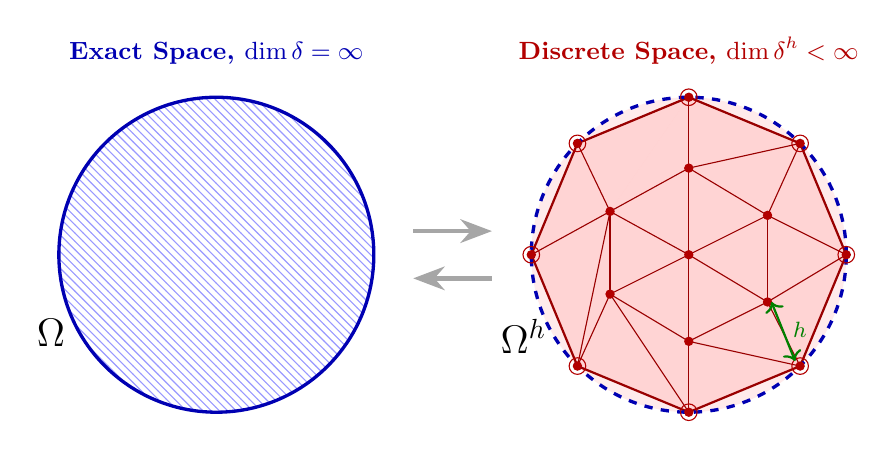
\begin{tikzpicture}[scale=1.]

    % =========================================================
    % LEFT PANEL: Exact space V
    % =========================================================
    \begin{scope}
        \begin{scope}
            \clip (0,0) circle (2);
            \fill[pattern=north west lines, pattern color=blue!40] 
                (-2.2,-2.2) rectangle (2.2,2.2);
        \end{scope}
        \draw[very thick, blue!70!black] (0,0) circle (2);
        \node[below=0.7cm] at (-2.1,0) {\Large $\Omega$};
        \node[above=2.3cm, blue!70!black, font=\small\bfseries] 
            at (0,0) {Exact Space, $\dim \delta = \infty$};
    \end{scope}

    % =========================================================
    % RIGHT PANEL: Discretized space V^h
    % All coordinates defined at TOP LEVEL of the tikzpicture
    % =========================================================
    
    % Shift origin manually for the right panel
    % Right panel center is at (6, 0)
    
    % --- Interior nodes (absolute coordinates) ---
    % (We add 6 to x to shift the panel)
    % C  = (6.0,  0.0)
    % N1 = (6.0,  1.1)
    % N2 = (7.0,  0.5)
    % N3 = (7.0, -0.6)
    % N4 = (6.0, -1.1)
    % N5 = (5.0, -0.5)
    % N6 = (5.0,  0.55)
    
    % --- Light fill of the right domain ---
    \begin{scope}
        \clip (6,0) circle (2);
        \fill[red!8] (3.8,-2.2) rectangle (8.2,2.2);
    \end{scope}
    
    % --- Filled triangles (drawn manually, no \foreach on coordinates) ---
    \fill[red!25, opacity=0.5] (6.0, 0.0) -- (6.0, 1.1) -- (7.0, 0.5) -- cycle;
    \fill[red!25, opacity=0.5] (6.0, 0.0) -- (7.0, 0.5) -- (7.0,-0.6) -- cycle;
    \fill[red!25, opacity=0.5] (6.0, 0.0) -- (7.0,-0.6) -- (6.0,-1.1) -- cycle;
    \fill[red!25, opacity=0.5] (6.0, 0.0) -- (6.0,-1.1) -- (5.0,-0.5) -- cycle;
    \fill[red!25, opacity=0.5] (6.0, 0.0) -- (5.0,-0.5) -- (5.0, 0.55) -- cycle;
    \fill[red!25, opacity=0.5] (6.0, 0.0) -- (5.0, 0.55) -- (6.0, 1.1) -- cycle;
    
    % --- Boundary triangles ---
    \fill[red!25, opacity=0.5] (6.0, 1.1) -- (6, 2) -- (7.414, 1.414) -- cycle;
    \fill[red!25, opacity=0.5] (6.0, 1.1) -- (7.414, 1.414) -- (7.0, 0.5) -- cycle;
    \fill[red!25, opacity=0.5] (7.0, 0.5) -- (7.414, 1.414) -- (8, 0) -- cycle;
    \fill[red!25, opacity=0.5] (7.0, 0.5) -- (8, 0) -- (7.0, -0.6) -- cycle;
    \fill[red!25, opacity=0.5] (7.0,-0.6) -- (8, 0) -- (7.414,-1.414) -- cycle;
    \fill[red!25, opacity=0.5] (7.0,-0.6) -- (7.414,-1.414) -- (6.0,-1.1) -- cycle;
    \fill[red!25, opacity=0.5] (6.0,-1.1) -- (7.414,-1.414) -- (6, -2) -- cycle;
    \fill[red!25, opacity=0.5] (6.0,-1.1) -- (6, -2) -- (5.0,-0.5) -- cycle;
    \fill[red!25, opacity=0.5] (5.0,-0.5) -- (6, -2) -- (4.586,-1.414) -- cycle;
    \fill[red!25, opacity=0.5] (5.0,-0.5) -- (4.586,-1.414) -- (5.0, 0.55) -- cycle;
    \fill[red!25, opacity=0.5] (5.0, 0.55) -- (4.586,-1.414) -- (4, 0) -- cycle;
    \fill[red!25, opacity=0.5] (5.0, 0.55) -- (4, 0) -- (4.586, 1.414) -- cycle;
    \fill[red!25, opacity=0.5] (5.0, 0.55) -- (4.586, 1.414) -- (6, 2) -- cycle;
    \fill[red!25, opacity=0.5] (5.0, 0.55) -- (6, 2) -- (6.0, 1.1) -- cycle;
    
    % --- Mesh edges ---
    \draw[red!60!black, thin] (6.0, 0.0) -- (6.0, 1.1);
    \draw[red!60!black, thin] (6.0, 0.0) -- (7.0, 0.5);
    \draw[red!60!black, thin] (6.0, 0.0) -- (7.0,-0.6);
    \draw[red!60!black, thin] (6.0, 0.0) -- (6.0,-1.1);
    \draw[red!60!black, thin] (6.0, 0.0) -- (5.0,-0.5);
    \draw[red!60!black, thin] (6.0, 0.0) -- (5.0, 0.55);
    
    \draw[red!60!black, thin] (6.0, 1.1) -- (7.0, 0.5);
    \draw[red!60!black, thin] (7.0, 0.5) -- (7.0,-0.6);
    \draw[red!60!black, thin] (7.0,-0.6) -- (6.0,-1.1);
    \draw[red!60!black, thin] (6.0,-1.1) -- (5.0,-0.5);
    \draw[red!60!black, thin] (5.0,-0.5) -- (5.0, 0.55);
    \draw[red!60!black, thin] (5.0, 0.55) -- (6.0, 1.1);
    
    % Boundary edges
    \draw[red!60!black, thin] (6.0, 1.1) -- (6, 2);
    \draw[red!60!black, thin] (6.0, 1.1) -- (7.414, 1.414);
    \draw[red!60!black, thin] (7.0, 0.5) -- (7.414, 1.414);
    \draw[red!60!black, thin] (7.0, 0.5) -- (8, 0);
    \draw[red!60!black, thin] (7.0,-0.6) -- (8, 0);
    \draw[red!60!black, thin] (7.0,-0.6) -- (7.414,-1.414);
    \draw[red!60!black, thin] (6.0,-1.1) -- (7.414,-1.414);
    \draw[red!60!black, thin] (6.0,-1.1) -- (6, -2);
    \draw[red!60!black, thin] (5.0,-0.5) -- (6, -2);
    \draw[red!60!black, thin] (5.0,-0.5) -- (4.586,-1.414);
    \draw[red!60!black, thin] (5.0, 0.55) -- (4.586,-1.414);
    \draw[red!60!black, thin] (5.0, 0.55) -- (4, 0);
    \draw[red!60!black, thin] (5.0, 0.55) -- (4.586, 1.414);
    \draw[red!60!black, thin] (6, 2) -- (4.586, 1.414);
    \draw[red!60!black, thin] (6, 2) -- (7.414, 1.414);
    
    % Polygonal boundary
    \draw[red!60!black, thick] (6,2) -- (7.414,1.414) -- (8,0) -- 
        (7.414,-1.414) -- (6,-2) -- (4.586,-1.414) -- (4,0) -- 
        (4.586,1.414) -- cycle;
    
    % Exact boundary (dashed)
    \draw[very thick, blue!70!black, dashed] (6,0) circle (2);
    
    % --- Nodes (drawn with explicit coordinates) ---
    \fill[red!70!black] (6.0, 0.0) circle (1.7pt);
    \fill[red!70!black] (6.0, 1.1) circle (1.7pt);
    \fill[red!70!black] (7.0, 0.5) circle (1.7pt);
    \fill[red!70!black] (7.0,-0.6) circle (1.7pt);
    \fill[red!70!black] (6.0,-1.1) circle (1.7pt);
    \fill[red!70!black] (5.0,-0.5) circle (1.7pt);
    \fill[red!70!black] (5.0, 0.55) circle (1.7pt);
    
    \foreach \x/\y in {6/2, 7.414/1.414, 8/0, 7.414/-1.414, 6/-2, 
                        4.586/-1.414, 4/0, 4.586/1.414} {
        \fill[red!70!black] (\x,\y) circle (1.7pt);
        \draw[red!70!black, thin] (\x,\y) circle (3pt);
    }
    
    % --- Labels ---
    \node[below=0.7cm] at (3.9,0) {\Large $\Omega^h$};
    \node[above=2.3cm, red!70!black, font=\small\bfseries] 
        at (6,0) {Discrete Space, $\dim \delta^h < \infty$};
    
    % --- Characteristic length h ---
    \draw[<->, thick, green!50!black] (7.05,-0.6) -- (7.35,-1.35);
    \node[right, font=\footnotesize, green!50!black] 
        at (7.2,-0.95) {$h$};

    % =========================================================
    % Arrow between panels
    % =========================================================
    \draw[-{Stealth[length=4mm, width=3mm]}, ultra thick, gray!70] 
        (2.5, 0.3) -- (3.5, 0.3);
    \draw[-{Stealth[length=4mm, width=3mm]}, ultra thick, gray!70] 
        (3.5, -0.3) -- (2.5, -0.3);

\end{tikzpicture}
\end{document}
